% 
% Submission to: http://wodes2014.lurpa.ens-cachan.fr/
% 
% \documentclass[a4paper,oneside]{article}
\documentclass[a4paper, 10pt, conference]{ieeeconf}
\IEEEoverridecommandlockouts
 % This command is only
  % needed if you want
  % to use the \thanks
  % command
\overrideIEEEmargins
% See the \addtolength command later in the file to balance the column lengths
% on the last page of the document

\usepackage[pdftex, pdftitle={DiagnosabilityVerification of Discrete-Event
Systems}, pdfauthor={Dmitry Myadzelets}, bookmarks=false,
% colorlinks=true, linkcolor=black
]{hyperref}

\usepackage{amsfonts, amssymb, amsmath} 
\usepackage{graphicx}
\usepackage{epstopdf}
\usepackage{tikz}
\usetikzlibrary{decorations.pathreplacing}
\usetikzlibrary{arrows,positioning,automata,shadows,fit,shapes}

\usepackage{algpseudocode}



\begin{document}

\title{Virtual Modules in Discrete-Event Systems: \\
Achieving Modular Diagnosability} 
\author{
	Dmitry Myadzelets$^{*,1,2}$
	, Andrea Paoli$^{1,3}$
	-- \today
	\thanks{$^{1}$Center for Research on Complex Automated Systems (CASY), DEI,
	University of Bologna, Viale Pepoli 3/2, 40123, Bologna, Italy}
		\thanks{$^{2}$E-mail: {dmitry.myadzelets@gmail.com}}
		\thanks{$^{3}$E-mail: {andrea.paoli@unibo.it}}
}
\maketitle

% To meet requirements of EU funding
% http://eacea.ec.europa.eu/about/eacea_logos_en.php "This project has been
% funded with support from the European Commission. This publication reflects
% the views only of the author, and the Commission cannot be held responsible
% for any use which may be made of the information contained therein."
% \begin{figure}[!b]
% \begin{tabular}{l p{60mm}}
%  	
\includegraphics[height=10mm]{EU_flag.eps}
%  	& \vspace{-10mm} \footnotesize
%  	$^{*}$With the support of the Erasmus Mundus Action 2 programme of the
%  	European Union.
% \end{tabular}
% \end{figure}

\begin{abstract}

\end{abstract}

\begin{keywords}
Discrete Event Systems, Modular Structure, Distributed Diagnosability
\end{keywords}

\newtheorem{theorem}{Theorem}
\newtheorem{definition}{Definition}
\newtheorem{lemma}{Lemma}
\newtheorem{assumption}{Assumption}
\newtheorem{corollary}{Corollary}
\newtheorem{example}{Example}
\newtheorem{algorithm}{Algorithm}


%%%%%%%%%%%%%%%%%%%%%%%%%%%%%%%%%%%%%%%%%%%%%%%%%%%%%%%%%%%%%%%%%%%%%%%%%%%%%%
\section{Introduction}

[Problem and literature]

[Summary of the ECC paper (Simplified, with 2 modules). Here we relaxing
assumptions\ldots]

Figure \ref{fig:curves} shows that the average size of a module grows while the
system's modules are composed together (we imply that each module is represented
by automata, and the size of a module is reflected by the number of states of
the correspondent automaton).
A shape of this curve depends mostly on the order the modules are taken for the
composition, but the initial point, when the system has maximal modularity, and
the final point, when all the modules are composed into one monolithic module,
remain the same. Assuming that the system is diagnosable, the average size of a
diagnoser grows much faster, since it is exponential with respect to the average
size of a module, in the worst case.
The amount of events, the diagnosers have to exchange among each other in order
to decide if a fault occurred, is decreasing. This reason the diagnosers require
less event for decision making is due to the fact that they become
self-sufficient, since the amount of observable events available for each
diagnoser without communications is growing. Thus, the events exchange rate
decreases down to the point where no communications is required to make a
decision about the faults occurrence. That is the point when the system becomes
modular diagnosable. The following composition of the modules does not affect
diagnosability, and leads only to the growth of the modules' and diagnosers'
sizes. In our approach, given a system with an initial modularity, we search for
a such point, when the system is modular diagnosable. If the system is
diagnosable, then this point can always be found. The modules correspondent to
that modularity we call virtual, since they are not composed in reality, and
used only to build diagnosers.

\begin{figure}
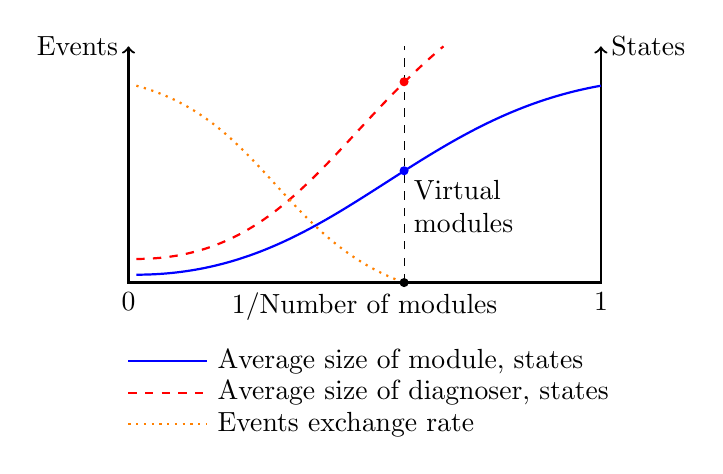
\begin{tikzpicture}
% \draw[help lines] (0,0) grid (5,3);
% Axis 
\draw [thick, <->] 
	(0,3) node[left]{Events} -- 
	(0,0) node[below]{0} -- 
	(6,0) node[below]{1} -- 
	(6,3) node[right]{States};
\node [below] at (3,0) {1/Number of modules};
% Curve of the average size of modules
\draw[blue, thick] (0.1,.1) to [out=0,in=-170] (6,2.5); 
% Curve of the average size of diagnosers
\draw[red, thick, dashed] (0.1,.3) to [out=0,in=-140] (4,3); 
% Curve of the amount of communication
\draw[orange, thick, dotted] (0.1,2.5) to [out=-15,in=160] (3.5,0); 
% Line of the point with virtual modularity
\draw[dashed] (3.5,0) -- (3.5,3);
% Point of virtual modularity  
\draw [fill] (3.5,0) circle [radius=0.05];
\draw [fill, blue] (3.5,1.42) circle[radius=0.05] 
	node[align=left, black, below right] {Virtual\\ modules}; 
\draw [fill, red] (3.5,2.55) circle [radius=0.05];
% Legend
\draw[blue, thick] (0,-1) -- (1,-1)
	node[black, right] {Average size of module, states};
\draw[red, thick, dashed] (0,-1.4) -- (1,-1.4)
	node[black, right] {Average size of diagnoser, states};
\draw[orange, thick, dotted] (0,-1.8) -- (1,-1.8) 
	node[black, right] {Events exchange rate};

\end{tikzpicture}
\caption{Changing of size of modules, diagnosers, and events exchange rate
with respect to the number of modules in the same system}
\label{fig:curves}
\end{figure}

[What is the new contribution]


%%%%%%%%%%%%%%%%%%%%%%%%%%%%%%%%%%%%%%%%%%%%%%%%%%%%%%%%%%%%%%%%%%%%%%%%%%%%%%
\section{Preliminaries}
\label{sec:Preliminaries}

\subsection{Notation}
The notation used in this document is the one in
\cite{cassandras_introduction_2010}.
Let $\Sigma$ be a finite set of events. A sequence of events is a string.
$\Sigma^*$ denotes a set of all finite strings over $\Sigma$.
$L\subseteq\Sigma^*$ is a language over $\Sigma$. Given strings $s$ and $t$,
$st$ is their concatenation. Given strings $s$ and $w$, $w$ is a prefix of $s$
if exists $t$ such that $wt = s$. Prefix closure of $L$, denoted by
$\overline{L}$ is a set of all prefixes of all the strings in $L$.
If $\overline{L} = L$ then $L$ is prefix-closed. The post language of $L$ after
a string $s$ is denoted as $L/s$, i.e. $L/s := \{t\mid st \in L\}$. We
write $\sigma \in s$ if the event $\sigma \in \Sigma$ appears in the string $s
\in \Sigma^*$. If $\{s\}$ is a singleton, we write $s$ for operations on
languages.

An automaton $G$ is a tuple $$G := \left< X,\Sigma,\delta,x_0, X_m \right>,$$
where $X$ is a set of states, $x_0 \in X$ is an initial state, $X_m \subseteq X$
is the set of marked states, and $\delta: X \times \Sigma \rightarrow X$ is the
transition function.
We say a language $L := \mathcal{L}(G)$ is generated or recognized by the
automaton $G$. In this paper we assume that for each language there is always a
correspondent automaton, and vice versa. The marked language $L_m \subseteq L$
is intended to make a part of the automaton's behaviour distinguishable in a
certain context.

Some events of DES can not be observed. To reflect that the set of events
$\Sigma$ is partitioned into disjointed sets of observable events $\Sigma_o$ and
not observable events $\Sigma_{ou}$, i.e. $\Sigma = \Sigma_o~\dot{\cup}~
\Sigma_{ou}$.
The $M: \Sigma^* \rightarrow \Sigma_o^*$ denotes the natural projection that
erases unobservable events.
% ; $\epsilon$ means the empty string. 
The correspondent inverse projection is $M^{-1}: \Sigma_o^* \rightarrow
2^{\Sigma^*}$.
If a set of events is partitioned into subsets, $\Sigma := \bigcup_i
\Sigma_{i} \mid i \in \mathbb{N}$, the natural projection over the partition
members is denoted as $M_i: \Sigma_i^* \rightarrow \Sigma_{i,o}^*$.

Let $I := \{1,2,\ldots,n\} \subset  \mathbb{N}$ be an index set. A system is
defined by a set of automata $\{G_{i \in I}\}$ and a correspondent set of
languages $\{L_{i \in I}\}$. We use the term \emph{local} in context of the
automata and languages from these sets. The \emph{global} language of the system
is defined by the parallel composition \cite{cassandras_introduction_2010} of
its local languages:
$L := \parallel_{i \in I} L_i$.
The natural projection is commonly defined over Kleene closure on event sets.
We restrict it, for simplicity of notation, to the system's languages as
follows: $P_i(L) := \{s\mid s\in L_{i}\}$, and $P_i^{-1}(L_{i}) := \{s \mid s
\in L\}, ~i \in I$.


\subsection{Adjacency graph}
A DES can be seen as a graph where its nodes represent the modules, and edges
reflect the fact that some modules are synchronized with each other. This
abstraction is often implicitly or explicitly used in approaches devoted to
diagnosability of modular systems. In our approach we denote such graph as the
\emph{adjacency graph}, formally defined as follows:
\begin{definition}
\label{def:graph_events}
Given $\{\Sigma_i \mid i \in I \}$, let $\mathcal{G} = \left<I, E\right>$ be an
undirected adjacency graph where $E \subseteq I \times
I$ such that 
$$(\forall i, j \in I)(i, j) \in E \Leftrightarrow 
	\Sigma_i \cap \Sigma_j \neq \emptyset \mid i \neq j.$$
\end{definition}
We extend this definition over languages.
\begin{definition}
\label{def:graph_languages}
The adjacency graph over a set of languages $\{L_i \subseteq \Sigma_i^* \mid i
\in I \}$ is a graph $\mathcal{G} = \left<I, E\right>$ where $E \subseteq I \times
I$ such that 
$$(\forall i, j \in I)(i, j) \in E \Leftrightarrow
	P_{i,j}^{-1}(L_i) \cap P_{i,j}^{-1}(L_j) \neq \emptyset \mid i \neq j, 
$$
where 
$P_{i,j} : (\Sigma_i \cup \Sigma_j)^* \rightarrow (\Sigma_i \cap \Sigma_j)^*$
, and  
$P_{i,j}^{-1}(s) := \{t \in (\Sigma_i \cup \Sigma_j)^* \mid P_{i,j}(t) = s\}$.
\end{definition}

By definition, the adjacency graph over $\{\Sigma_i\}$ is a supergraph for any
graph over $\{L_i \subseteq \Sigma_i\}$, and any adjacency graph over $\{L'_i
\subseteq L_i\}$ is a subgraph of the adjacency graph over $\{L_i\}$.

% Recall that in graph theory a simple path is a path in a graph which does not
% have repeating vertices.


%%%%%%%%%%%%%%%%%%%%%%%%%%%%%%%%%%%%%%%%%%%%%%%%%%%%%%%%%%%%%%%%%%%%%%%%%%%%%%
\section{General form of the approach}
\label{sec:General}

[Formal problem definition]
[Figure of modular and decentralized diagnosability (from the presentation)]

In the first article we introduced an analysis of a trivial system of two
languages, with conditions for the both languages, when one language makes the
system diagnosable if the other language is not locally diagnosable.
The conditions are sufficient, and they also are necessary if we assume that the
local languages are not affected by concurrency, i.e. $L_i = P_i(L)$. Some of
the conditions require one language to have common events with the other one. In
general, a system consists of many modules, and a language which is not
diagnosable locally may have no common events with a language which can
potentially change diagnosability, but have common events with other languages.
In this case one can compose all the other languages with the faulty language,
reducing the system to the form of the trivial case. A formal description of
such approach is given below.

The setup for the problem is following. Let a system be defined as a set of
local languages $S := \{L_{i\in I}\}$, and let faulty behaviours be defined for
any $i \in I$, i.e. each language $L_i$ can be disjoint into faulty and
non-faulty sublanguages: $L_{i,f}$ and $L_{i,nf}$. We assume that $(\forall i
\in I)\left[ L_i = P_i(L)\right]$.

First, we recall the definition of diagnosability of virtual modules. Let $J$ be
a partition of $I$. Given the system $S$, $J$ and set of observable
projections $\{M_j := \Sigma_j^* \rightarrow \Sigma_{j,o}^* \mid j \in J \}$
where $\Sigma_j := \bigcup_i \Sigma_i,~ 
	\Sigma_{j,o} := \bigcup_i \Sigma_{i,o} \mid 
	i\in j$. 
The system is modularly diagnosable with respect to $J$ and $\{M_j\}$ 
if the following holds:
\begin{equation}
	\begin{array}{l}
		\forall(i \in I, s \in L_{i,f}, t \in L_{i,f}/s)
		\\
		(\exists n \in \mathbb{N})
		(|t| \geq n)
		\\
		\left[ M_j(P_i^{-1}(st)) \cap M_j(P_i^{-1}(L_{i,nf})) = \emptyset \right].
	\end{array}
\end{equation}
The definition requires each fault originated in any language of the subset $j$
to be diagnosed observing only events of the languages from the same subset $j$.
However, the languages $L_j$ are not given, and do not have to be necessary
constructed. That is why we use the term \emph{virtual module} as a synonym for
the subset $j$.

Second, we recall Lemma 2 of the first article, and rewrite it for an arbitrary
couple of languages as follows.

\begin{lemma}
Given a tuple $\left< L_i, L_j, s, u\right> \mid i, j \in \mathbb{N}, i\neq j$,
where $L_i, L_j$ are languages, and $s, u \in L_i$. The strings $s, u$ are
distinguished in the language $L_i \parallel L_j$, if for the string $s$ exists
an adjacent observable support $K_j \subseteq L_j$ which satisfies the
condition:
\end{lemma} 
\begin{equation}
\label{con:distinquished}
	\begin{array}{l}
	 	(\forall t \in K_j)
	 	(\exists \sigma \in t \mid \sigma \in \Sigma_i \cap \Sigma_j)
	 	(\sigma \not \in u)
	 	\\
	 	(\forall w\sigma \in \overline{t})
	 	[M_j(t / w\sigma) \neq \emptyset].
	\end{array}
\end{equation}
% where $M'_j: (\Sigma_i \cup \Sigma_j)^* \rightarrow (\Sigma_{j,o}\backslash
% \Sigma_i)^*$.
Informally, the lemma imposes a requirement for the string $s$ to have an
observable support in another language, which guaranties that we can observe some
events in that language before any continuation of the string $s$.
Then, the lemma defines a condition which allows us to distinguish these
observations from the observation of the string $u$.

Now, we rewrite Lemma 3 from the first article in the context of our setup, as
follows:
\begin{lemma}
\label{lem:virtual_module_is_diagnosable}
Given a set of languages $j \in J$, the virtual module $j$ is diagnosable with
respect to $M_j$ if:
\end{lemma}
\begin{equation}
	\begin{array}{l}
% 		(\forall i \in j, s \in L_{i,f}, t \in L_i \backslash \overline{L_{i,f}})
		(\forall i \in j, 
			s \in P_i^{-1}(L_{i,f}), 
			t \in P_i^{-1}(L_{i,nf}))
% 			t \in P_i^{-1}(L_i) \backslash \overline{P_i^{-1}(L_{i,f})})
		\\
		(\exists k \in j \mid k \neq i) \textrm{ and }
		\\
		\textrm{condition (\ref{con:distinquished}) holds for at least one of
		the tuples:}
		\\
		\left<P_i^{-1}(L_i), L_k, s, t \right>,
		\left<P_i^{-1}(L_i), L_k, t, s \right>.
	\end{array}
\end{equation}
The lemma implies that the virtual module is diagnosable if we can distinguish
all faulty strings from all non-faulty strings. 
% excluding all prefixies of the faulty strings
% Note, that exclusion of the prefixes comes from fact that the non-compositional
% analysis is used.
From the lemma it can be seen that for one faulty sublanguage there can be a
subset of languages with observable supports, satisfying the conditions. In
order to make the system modularly diagnosable, thus, one needs to find a
relevant partition, with a desired distribution of modules. It worth to note,
that the partitioning implies that languages with faults are in subsets with the
languages which have observable events. Thus, other languages which have no
faults and have no observable events, as well the languages with observations
which have no effect for the diagnosability property, will be in other subsets.
Since it is enough to pick just one module satisfying the conditions, we
propose a procedure for this task, in the next section.

\section{Algorithm to choose a module with observable support}
Assume that the objective function is to have the number of modules in the
system as many as possible, i.e. to have the maximal cardinality of the
partition $J$.
Given an initial set of languages, let rank of $J$ be equal to 0, i.e. $|J| =
|I|$. Let $F$ denotes the subset of languages with faults, and $M$ denotes the
subset of languages with correspondent observable supports.
Assume that it is always possible to make the system modularly diagnosable with
respect to some virtual modules. Then we know that $(\forall f \in F)~\exists m
\in M$. Let $F \cap M = \emptyset$ and $|M| \geq |F|$. Then, to make the system
modularly diagnosable it is required, in the worst case, $|F|$ members of $M$.
Thus, the cardinality of the systems with virtual modules, i.e. the cardinality
of the partition, in the worst case is:
\begin{equation}
	\min |J| = |I| - |F|.
\end{equation}
Let $M \subseteq F$. Then, the cardinality of the partition in the best case
is:
\begin{equation}
	\max |J| = |I| - \left(
		\left\lfloor \frac{|F|}{2} \right\rfloor + \textrm{mod} \frac{|F|}{2}
		\right). 
\end{equation}

As can be seen from the above, in order to maximize the number of modules while
making the virtual modules, we should consider, firstly, the modules which
themselves have faults. We propose a procedure for the given objective function
as follows:

Given the system $S$ of cardinality $|I|$, the subset $F
\subseteq I$ of modules with faults, such that any $f\in F$ is not diagnosable
locally, the subset $M \subseteq I$ of modules with observable supports, such
that $(\forall f \in F)~\{m \in M\}\neq \emptyset$. In order to make the system
diagnosable by minimal number of virtual modules: 
\begin{enumerate}
  \item Initially set the partition $J$ of $I$ such that the rank of $J$ is
  equal to 0;
  \item $(\forall j \in J, f \in j)$ update $j$ as follows: 
  	$j := j \cup \{m \in M \cap F\}$ if $M \cap F \neq \emptyset$,
 $j := j \cup \{m \in M\}$ otherwise, where $\{m\}$ is a singleton of the
 arbitrary chosen observable support for the given $f$, such that the new $j$
 is locally diagnosable; exclude $m$ from $k \in J \mid k \neq j$, and remove
 $k$ from $J$ if $k=\emptyset$.
\end{enumerate} 
The order the observable supports are verified in the procedure guaranties that
we consider, firstly, the languages which themselves contain the faulty
sublanguages, thus maximizing the number of virtual modules in the system.

It worth to note that the above algorithm can be augmented by additional
criteria aimed, for instance, to decrease computational burden.

% The objective function discribes a combinatorial optimisation problem, which can
% be solved by linear programming methods.

\section{Co-faulty language}

Assume that given a language with faulty behaviour and a language which has an
observable support. It is now required to verify if the observable support is
either for the faulty or non-faulty sublanguages. If it is true, then the
correspondent modules can be composed into a virtual module.
According to the Lemma \ref{lem:virtual_module_is_diagnosable}, in order to
decide if the virtual module is diagnosable we need to verify the necessary
conditions for all the strings $P_i^{-1}(L_{i,f})$ and $P_i^{-1}(L_{i,nf})$,
projected to the local languages of other modules.

[Here should be a motivation for the definition of the co-faulty sublanguage.]

\begin{definition}
\label{def:co-faulty}
Given $i, j \in I$, $L_{i,f} \subseteq L_i$,
we say that a sublanguage $L_{j,cf} \subseteq L_j$ is \emph{co-faulty} with
respect to $L_{i,f}$ if 
$$
	(\forall s \in L_{j,cf})(\forall t \in P_i[P_j^{-1}(s)])
	\left[
		t \in L_{i,f} \land t \not \in L_{i,nf}   
	\right],
$$ 
and a sublanguage $L_{j,cnf} \subseteq L_j$ is
\emph{co-non-faulty} with respect to $L_{i,nf}$ if 
$$
	(\forall s \in L_{j,cnf})(\forall t \in P_i[P_j^{-1}(s)])
	\left[
		t \not \in L_{i,f} \land t \in L_{i,nf}   
	\right].
$$ 
\end{definition}

In words, the co-faulty sublanguage is a sublanguage which satisfies two
conditions:
a) it is the sublanguage of projection of the global faulty language
to the local language; b) the sublanguage is not co-non-faulty.
Similarly, the co-non-faulty sublanguage is a sublanguage which satisfies
conditions:
a) it is the sublanguage of projection of the global non-faulty language
to the local language; b) the sublanguage is not co-faulty.

\begin{lemma}
\label{lem:empty_co_if_no_common}  
Given a language $L_j\mid j \in I$, its co-faulty and
co-non-faulty sublanguages are empty, if the language has no common events in
its strings, i.e
$$P_{\Sigma_j \rightarrow \bigcap_{i\neq j}^I \Sigma_i}(L_i) = \emptyset.$$
\end{lemma}

We skip the proof due to its triviality. 

Given global faulty and non-faulty sublanguages, one can compute the local
co-faulty sublanguage as follows:
\begin{equation}
\label{eq:co-faulty_from_global}
	\begin{array}{l}
		L_{j,cf} := P_j(L_f) \backslash P_j(L_{nf}),\\ 
		L_{j,cnf} := P_j(L_{nf}) \backslash P_j(L_{f}).	
	\end{array}
\end{equation}
However, we are interested to compute a local co-faulty
language without computing the global language. Since the global
faulty sublanguage is define as
\begin{equation}
\label{eq:co-faulty_from_locals}
	L_f := P_i^{-1}(L_{i,f}) \cap \bigcap_{k\neq
	i}^I P_k^{-1}(L_k),
\end{equation}
then, by substituting the global language in \ref{eq:co-faulty_from_global} by
\ref{eq:co-faulty_from_locals}, and by mathematical induction, the co-faulty
sublanguage of an arbitrary module can be computed as follows:
% \begin{equation}
% 	\begin{array}{ll}
% 		L_{j,cf} := 
% 		&
% 		\bigcap_k^I P_j[P_k^{-1}(L_{k,cf}) \cap P_i^{-1}(L_{i,f})] 
% 		\backslash \\
% 		&
% 		\bigcap_k^I P_j[P_k^{-1}(L_{k,cnf}) \cap P_i^{-1}(L_{i,nf})],
% 		\\ & \textrm{where } i\neq j\neq k \in I.
% 	\end{array}
% \end{equation}
\begin{equation}
\label{eq:co-faulty_iterative_w_faulty}
	\begin{array}{l}
		L_{j,cf} := 
		\\
		P_j\Big(P_j^{-1}(L_j) \cap P_i^{-1}(L_{i,f})\cap 
		\bigcap_k^I P_k^{-1}(L_{k,cf})\Big) \backslash 
		\\
		P_j\Big(P_j^{-1}(L_j) \cap P_i^{-1}(L_{i,nf})\cap 
		\bigcap_k^I P_k^{-1}(L_{k,cnf})\Big),
		\\ 
		\textrm{where } i\neq j\neq k \in I.
	\end{array}
\end{equation}

According to Definition \ref{def:co-faulty}, any faulty language is co-faulty to
itself. This fact allows us to simplify equation
\ref{eq:co-faulty_iterative_w_faulty}, and rewrite is as follows:

\begin{equation}
\label{}
	\begin{array}{l}
		L_{j,cf} := 
		\\
		P_j\Big(P_j^{-1}(L_j) \cap 
		\bigcap_i^I P_i^{-1}(L_{i,cf})\Big) \backslash 
		\\
		P_j\Big(P_j^{-1}(L_j) \cap 
		\bigcap_i^I P_i^{-1}(L_{i,cnf})\Big),
		\\ 
		\textrm{where } i\neq j\in I.
	\end{array}
\end{equation}


Below we present an algorithm which, given a module with the co-faulty
sublanguage defined, computes the co-faulty languages of an adjacent module.

% In the following, when we assume that statements for co-faulty sublanguages also
% valid for co-non-faulty sublanguages.


% By definition, any faulty sublanguage is co-faulty with respect to itself.
% We use this property to establish relations  
% is used in the following lemma which establishes relation
% of co-faulty languages.
% 
% 
% 
% \begin{lemma}
% \label{lem:co-faulty-if-path}
% Given a set of languages $\{L_i \subseteq \Sigma_i^* \mid i \in I \}$ and the 
% adjacency graph $\mathcal{G}$ over this set. Any two vertexes $i, j \in I$,
% connected in the graph $\mathcal{G}$, also connected in the subgraph
% $\mathcal{G}_f$ over the set of co-faulty sublanguages $\{L_{i,cf}\}$, only if
% $$
% .
% $$
% Given $L_{i,f} \mid i \in I$ and set $\{L_{j,cf} \subseteq L_j \mid j \in J
% \subseteq I, j \neq i\}$ where $L_{j,cf}$ is co-faulty with respect to $L_{i,f}$. 
% For any $j \in J$ the $L_{j,cf}$ is not empty only if exists a path between $i$
% and $j$ in the adjacency graph $\mathcal{G}$ over languages.
% \end{lemma}

% \begin{proof} 
% Trivially, by induction from the definition of parallel composition of automata
% as a natural representation of parallel composition for languages.
% % (Sketch) 
% % Let $I = \{i, j\}$ and a faulty non empty sublanguage
% % $L_{i,f} \subseteq L_i$. Assume that $L_{j,cf} \subseteq L_j$ is not
% % empty, and there is no path between $i$ and $j$ in the graph, i.e.
% % $\Sigma_i \cap \Sigma_j = \emptyset$. \ldots by properties of intersection of
% % inverse projections (parallel composition).
% \end{proof}

\begin{algorithm} Computing the co-faulty and co-non-faulty languages of an
adjacent module.
\label{alg:partial_co_faulty}
\begin{algorithmic}[1]
	\Require $L_i, L_{i,cf}, L_{i,cnf}, L_j$
	\State $\Sigma_c \leftarrow \Sigma_i \cap \Sigma_j$ 
		\label{alg:pcf_get_common}
	\State $F \leftarrow P_{\Sigma_i \rightarrow \Sigma_c}(L_{i,cf})$
		\label{alg:pcf_get_common_f}
	\State $N \leftarrow P_{\Sigma_i \rightarrow \Sigma_c}(L_{i,cnf})$
		\label{alg:pcf_get_common_n}
	\State $K \leftarrow F \cap N$
		\label{alg:pcf_get_fn}
	\State $F \leftarrow F\backslash K$
		\label{alg:pcf_get_f}
	\State $N \leftarrow N\backslash K$
		\label{alg:pcf_get_n}
	\State $L_{j,cf} \leftarrow 
		(P_{\Sigma_j \rightarrow \Sigma_c}^{-1}(F)) \cap L_j$
		\label{alg:pcf_get_cf}
	\State $L_{j,cnf} \leftarrow 
		(P_{\Sigma_j \rightarrow \Sigma_c}^{-1}(N)) \cap L_j$
		\label{alg:pcf_get_cnf}
	\\
	\Return $L_{j,cf}, L_{j,cnf}$
\end{algorithmic}
\end{algorithm}

At the steps \ref{alg:pcf_get_common_f} and \ref{alg:pcf_get_common_n} of the
above algorithm we compute projections of known faulty and non-faulty languages.
Note, that natural projection operation preserves faulty property of languages,
as well as construction of correspondent deterministic automata. The both
languages $L_{i,cf}$ and $L_{i,cnf}$ are not prefix-closed, in general. Then,
their projections $F$ and $N$, with respect to the common events, may be not
prefix-closed either. At the step \ref{alg:pcf_get_fn} the prefix common to the
$F$ and $N$ is computed. Then, at the steps \ref{alg:pcf_get_f} and
\ref{alg:pcf_get_n} we update languages subtracting their common prefix.
Finally, we compute co-faulty and co-non-faulty languages for the adjacent
module. In this sequence of operations at the steps
\ref{alg:pcf_get_common_f}--\ref{alg:pcf_get_cnf} new automata for the
correspondent languages are constructed or modified, and all the operations can
be performed using standard software libraries.

Note, that the the Algorithm \ref{alg:partial_co_faulty} returns the co-faulty
sublanguage of the module $j$ which is co-faulty with respect to only the module
$i$, i.e. it is computed only partially. According to
(\ref{eq:co-faulty_iterative_w_faulty}), in order to compute the full co-faulty
sublanguage, we need to iterate over all the co-faulty sublanguages.



%%%%%%%%%%%%%%%%%%%%%%%%%%%%%%%%%%%%%%%%%%%%%%%%%%%%%%%%%%%%%%%%%%%%%%%%%%%%%%
% \section{Review of existing approaches}
% 
% The work \cite{su_global_2005} presents an algorithm named \emph{Computational
% Procedure for Global Consistency (CPGS)} to find the \emph{supremal
% global support}. Given a system 
% $\{ L_i \mid i \in I \subset \mathbb{N} \}$ 
% and its projections $\{ M_i \}$, the supremal global support is
% \begin{equation}
% 	Sup\Gamma = \{ P_i(\parallel M_i^{-1}M_i(L_i))\}.
% \end{equation}
% Informally, a string of a local language is in the global support if the string
% satisfies the conditions:
% \begin{enumerate}
%   \item the string contains observable events;
%   \item the string is not blocked in the global language. 
% \end{enumerate}
% Supremum implies that all the strings satisfying the above conditions have
% been found.
% 
% In words, the CPGS algorithm consequently computes the projection to the common
% events and then the parallel composition of this projection with a next module.
% Thus, the last language in the sequence is equal to $P_i(L)$. The above
% procedure is repeated with each module placed as the final in the sequence.
% 
% The order the modules are placed in the sequence for the algorithm may be
% random. Since here only common events cause growth of the composed language,
% intuitively, the ordering should be done with respect to them. Indeed, the
% article presents a heuristic ordering procedure for that, and introduces some
% parameters described below.
% 
% The first parameter represents the space complexity of parallel composition of
% two languages as follows:
% \begin{equation}
% 	A_{i,j} = \frac{| X_i \parallel X_j |}{|X_i|\times |X_j|}.
% \end{equation}
% It is the ratio of the minimal state space cardinality of the actual parallel
% composition result to the state space cardinality of the composition in the
% worst case.
% 
% The second parameter represents the space complexity of natural projection with
% respect to the events common for two languages:
% \begin{equation}
% 	B_{i,j} = \frac{
% 		| P_{\Sigma_i \cup \Sigma_j \rightarrow \Sigma_i \cap \Sigma_j}
% 		(X_i \parallel X_j) |}
% 		{| X_i \parallel X_j |}.
% \end{equation}
% It is the ratio of the minimal state space cardinality of the projection to the
% state space cardinality of the original language.
% 
% The lower the parameter $A$ the higher the coupling of two modules, i.e. more
% common events the modules have, and less memory is required for the computation
% of the parallel composition. Hence, we are interested to minimize $A$. The lower
% parameter $B$ implies less memory for the result of the projection. However,
% trying to minimize $B$ can lead to the increasing of $A$. Thus, the authors
% minimize both $A$ and $B$. Since at each step of the algorithm only one module is
% selected, the parameters can not be minimized independently. Therefore, the
% product of $A$ and $B$ was chosen to be minimized:
% \begin{equation}
% 	C = A \times B = 
% 		\frac{| P_{\Sigma_i \cup \Sigma_j \rightarrow \Sigma_i \cap \Sigma_j}
% 		(X_i \parallel X_j) |}
% 		{|X_i|\times |X_j|}.
% \end{equation}
% 
% In computer science the algorithm the authors use is called \emph{greedy
% algorithm}. Here it starts with a random module, and makes a local optimal
% choice based on the value of parameters $C$ calculated for the candidate set.
% The candidate set includes all the neighbor modules except the goal module. If
% the set of neighbors is empty then it includes all unprocessed modules except
% the goal module. The algorithm finishes after no any but the goal module can be
% included to the candidate set.
% 
% The time complexity of the algorithm is $O(n^2)$. It requires $|X|^n$ state
% space in the worst case, when a goal module splits the coupling graph into
% separate parts (star shape). 
% % However, the space complexity can be impoved up to $n|X|$ if the splitted parts
% % are processed separately first, and then the goal module is processed with all
% % of them. << Too BIG complexity difference. Check it twice!

\begin{algorithm} Computing all co-faulty and co-non-faulty languages of
all the modules.
\label{alg:full_co_faulty}
\begin{algorithmic}[1]
	\Require A faulty module $i\in I$, $\{L_j\mid j \in I\}$
	\State $stack \leftarrow i$
	\While{$stack \neq \emptyset$}
		\State $i \leftarrow stack$
		\ForAll{$j \in I \mid j \textrm{ is adjacent to } i$}
			\State $\Sigma_c \leftarrow \Sigma_i \cap \Sigma_j$ 
			\State $F_i \leftarrow P_{\Sigma_i \rightarrow \Sigma_c}(L_{i,cf})$
			\State $F_j \leftarrow P_{\Sigma_j \rightarrow \Sigma_c}(L_{j,cf})$
			\State $N_j \leftarrow P_{\Sigma_j \rightarrow \Sigma_c}(L_{j,cnf})$
			\State $K \leftarrow F \cap N$
			\If{$F_i \cap \overline{F_j}\backslash K_j \neq \emptyset$}
				\State update $F_i$
				\State $stack \leftarrow j$ 
			\EndIf
		\EndFor
	\EndWhile
	\ForAll{$j \in I$}
		\State $L_{j,cf}:=(P_{\Sigma_j \rightarrow \Sigma_c}^{-1}(F_j)) \cap L_j$
	\EndFor
	\\
	\Return $\{L_{j,cf}, L_{j,cnf}\}$
\end{algorithmic}
\end{algorithm}

%%%%%%%%%%%%%%%%%%%%%%%%%%%%%%%%%%%%%%%%%%%%%%%%%%%%%%%%%%%%%%%%%%%%%%%%%%%%%%%
\section{Algorithm to decide diagnosability}
\label{sec:Algorithm}

\begin{enumerate}
  \item Starting from the faulty module, compute co-faulty and co-non-faulty
  local sublanguages. Make a subgraph $\mathcal{G}_f$ of the adjacency graph
  $\mathcal{G}$, removing nodes where modules have neither a co-faulty nor a
  co-non-faulty sublanguage.
  
  \item Get a subset of modules where the co-faulty or co-non-faulty
  sublanguages have observable events. Mark such nodes on the graph
  $\mathcal{G}_f$.
  
  \item If there is a path in the graph from the faulty module to at least one
  not marked node, then report that the system is not diagnosable (implies that
  that there is a indeterminate cycle, under assumption that the languages are
  live), continue otherwise.
  
  \item Track observable faulty and non-faulty paths along the nodes of the
  graph $\mathcal{G}_f$, checking if indistinguishable traces disappear. Each
  time a trace brakes due to an observable event, mark the node which has this
  event as a member for the virtual module. If all the paths are broken, then
  report that the system is diagnosable and return the set of nodes for the
  virtual module.
\end{enumerate}


%%%%%%%%%%%%%%%%%%%%%%%%%%%%%%%%%%%%%%%%%%%%%%%%%%%%%%%%%%%%%%%%%%%%%%%%%%%%%%%
\section{Example}
\label{sec:Example}


%%%%%%%%%%%%%%%%%%%%%%%%%%%%%%%%%%%%%%%%%%%%%%%%%%%%%%%%%%%%%%%%%%%%%%%%%%%%%%%
\section{Conclusions}
\label{sec:Conclusions}


\bibliographystyle{IEEEtran}
\bibliography{References}


\end{document}